\documentclass{../../../oss-classkick}
\begin{document}
\genheader

\gentitle{2}{MAGNETISM}

\genmultidirections

\gengravity

\raggedcolumns
\begin{multicols*}{2}

  \begin{enumerate}[leftmargin=18pt]
  \item  An electron is moving downward toward the bottom of the page when
    it passes through a region of magnetic field, as shown in the figure by
    the shaded area. The electron travels along a path that takes it through
    the spot marked $X$. The gravitational force on the electron is very
    small. What is the direction of the magnetic field?
    \begin{center}
      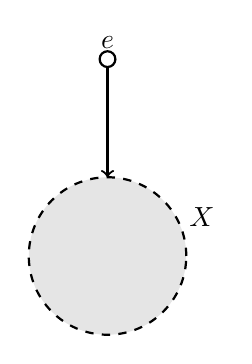
\begin{tikzpicture}
        \draw[thick,dashed,fill=gray!20](0,0) circle(1);
        \node at (1.2,.5) {$X$};
        \draw[thick](0,2.5) circle(.1) node[above]{$e$};
        \draw[thick,->](0,2.4)--(0,1);
      \end{tikzpicture}
    \end{center}
    \begin{enumerate}[nosep,leftmargin=18pt,label=(\Alph*)]
    \item Toward the bottom of the page
    \item Toward the top of the page
    \item Out of the page
    \item Into the page
    \end{enumerate}
    \vspace{.7in}
    
  \item Two long parallel wires carry currents ($I_A$ and $I_B$), as shown in
    the figure. Current $I_A$ in the left wire is twice that of current $I_B$ in
    the right wire. The magnetic force on the right wire is $F$. What is the
    magnetic force on the left wire in terms of $F$?
    \begin{center}
      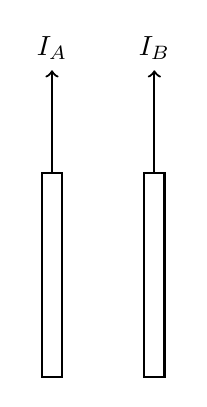
\begin{tikzpicture}[scale=1.3]
        \begin{scope}[thick]
          \draw(0,0) rectangle(.2,2);
          \draw(1,0) rectangle(1.2,2);
          \draw[->](.1,2)--(.1,3) node[above]{$I_A$};
          \draw[->](1.1,2)--(1.1,3) node[above]{$I_B$};
        \end{scope}
      \end{tikzpicture}
    \end{center}
    \begin{enumerate}[nosep,leftmargin=18pt,label=(\Alph*)]
    \item $F$ in the same direction
    \item $F$ in the opposite direction
    \item $F/2$ in the same direction
    \item $F/2$ in the opposite direction
    \end{enumerate}
    \vspace{.7in}
    
  \item An iron magnet is broken in half at the midpoint between its north
    andsouth ends. What is the result?
    \begin{enumerate}[nosep,leftmargin=18pt,label=(\Alph*)]
    \item A separate north pole and south pole, each with the same
      magnetic strength as the original magnet
    \item A separate north pole and south pole, each with half the magnetic
      strength of the original magnet 
    \item Two separate north-south magnets, each with the same magnetic
      strength as the original magnet
    \item Two separate north-south magnets, each with half the magnetic
      strength of the original magnet
    \end{enumerate}
    \vspace{.7in}
    \columnbreak

  \item The figure below shows the microscopic dipoles inside two metal objects.
    Copper is diamagnetic. Iron is ferromagnetic. Which of the following
    best depicts the microscopic internal dipole position when the objects
    are placed in a strong, external magnetic field directed toward the top
    of the page?
    \begin{center}
      \pic{.15}{copper-iron}

      \pic{.45}{domains}
    \end{center}
    \vspace{.7in}
    
  \item A magnetic field, directed into the page, is placed between two charged
    capacitor plates, as shown in the figure. The magnetic and electric fields
    are adjusted so a proton moving at a velocity of $v$ will pass straight
    through the fields. The speed of the proton is doubled to $2v$. Which of the
    following force diagrams most accurately depicts the forces acting on the
    proton when traveling at $2v$?
    \begin{center}
      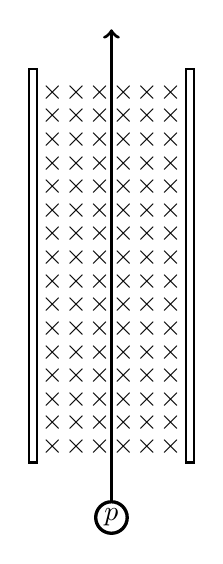
\begin{tikzpicture}
        \begin{scope}[thick]
          \draw(0,0) rectangle(.1,5);
          \draw(2,0) rectangle(2.1,5);
          \foreach\x in {.3,.6,...,2}{
            \foreach\y in {.2,.5,...,5} \node at (\x,\y) {$\times$};
          }
          \draw[very thick,->](1.05,-.5)--(1.05,5.5);
          \draw[very thick](1.05,-.7) circle(.2) node{$p$};
        \end{scope}
      \end{tikzpicture}
    \end{center}
    \begin{enumerate}[nosep,leftmargin=18pt,label=(\Alph*)]
    \item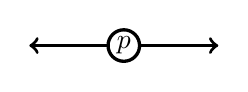
\begin{tikzpicture}
      \draw[very thick](0,0) circle(.2) node{$p$};
      \draw[very thick,->](.2,0)--(1.2,0);
      \draw[very thick,->](-.2,0)--(-1.2,0);
    \end{tikzpicture}

    \item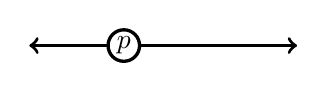
\begin{tikzpicture}
      \draw[very thick](0,0) circle(.2) node{$p$};
      \draw[very thick,->](.2,0)--(2.2,0);
      \draw[very thick,->](-.2,0)--(-1.2,0);
    \end{tikzpicture}

    \item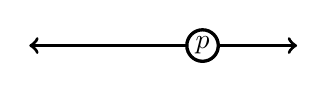
\begin{tikzpicture}
      \draw[very thick](0,0) circle(.2) node{$p$};
      \draw[very thick,->](.2,0)--(1.2,0);
      \draw[very thick,->](-.2,0)--(-2.2,0);
    \end{tikzpicture}

    \item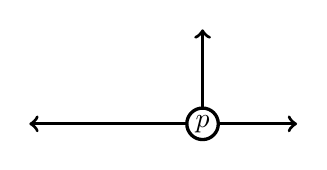
\begin{tikzpicture}
      \draw[very thick](0,0) circle(.2) node{$p$};
      \draw[very thick,->](.2,0)--(1.2,0);
      \draw[very thick,->](-.2,0)--(-2.2,0);
      \draw[very thick,->](0,.2)--(0,1.2);
    \end{tikzpicture}
    \end{enumerate}
    \vspace{.7in}
    \columnbreak
    
  \item Which of the following is true concerning the force on the
    current-carrying wire due to the electron?
    \begin{center}
      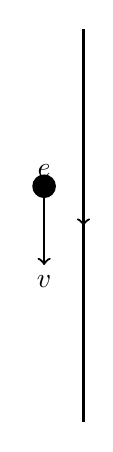
\begin{tikzpicture}
        \draw[thick,->](0,5)--(0,2.5);
        \draw[thick](0,3)--(0,0);
        \fill(-.5,3) circle(.15) node[above] {$e$};
        \draw[thick,->](-.5,3)--(-.5,2) node[below]{$v$};
      \end{tikzpicture}
    \end{center}
    \begin{enumerate}[nosep,leftmargin=18pt,label=(\Alph*)]
    \item The force is directed toward the right.
    \item The force is directed toward the left.
    \item The force is directed into the page.
    \item There is no force on the current-carrying wire due to the electron.
    \end{enumerate}
  \end{enumerate}
  \textbf{Questions \ref{q:2wires1}--\ref{q:2wires2}}
  
  Two wires carry currents $2A$ and $4A$ in the directions shown. Point $P$ is a
  distance $r$ from the wire carrying $2A$, and a distance $2r$ from the wire
  carrying $4A$.
  \begin{center}
    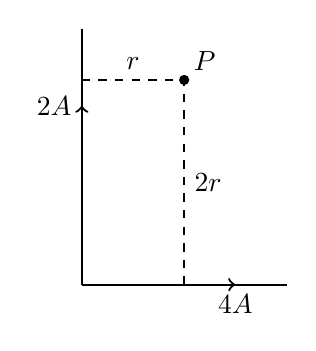
\begin{tikzpicture}[scale=1.3]
      \draw[thick](0,0)--(2,0);
      \draw[thick,->](0,0)--(1.5,0) node[below]{$4A$};
      \draw[thick](0,0)--(0,2.5);
      \draw[thick,->](0,0)--(0,1.75) node[left]{$2A$};
      \draw[thick,dashed](0,2)--(1,2)node[midway,above]{$r$}
      --(1,0) node[midway,right]{$2r$};
      \fill[black](1,2) circle(.05) node[above right]{$P$};
    \end{tikzpicture}
  \end{center}
  \begin{enumerate}[leftmargin=18pt,resume]
  \item Which of the following statements is true?
    \begin{enumerate}[noitemsep,topsep=0pt,leftmargin=18pt,label=(\Alph*)]
    \item The magnetic field produced at point $P$ by the wire carrying $2A$ is
      greater than the magnetic field produced at point $P$ by the wire
      carrying $4A$, but opposite in direction.
    \item The magnetic field produced at point $P$ by the wire carrying $2A$ is
      less than the magnetic field produced at point $P$ by the wire
      carrying $4A$, and in the same direction.
    \item The magnetic field produced at point $P$ by the wire carrying $2A$ is
      equal to the magnetic field produced at point $P$ by the wire
      carrying $4A$, but opposite in direction.
    \item The magnetic field produced at point $P$ by the wire carrying $2A$ is
      equal to the magnetic field produced at point $P$ by the wire
      carrying $4A$, and in the same direction.
    \item The magnetic field produced at point $P$ by the wire carrying $2A$ is
      greater than the magnetic field produced at point $P$ by the wire
      carrying $4A$, and in the same direction.
    \end{enumerate}
    \label{q:2wires1}
    \vspace{.7in}
    
  \item The magnitude of the resultant magnetic field at point $P$ due to the
    current in the two wires is
    \begin{enumerate}[nosep,leftmargin=18pt,label=(\Alph*)]
    \item zero
    \item $\displaystyle\frac{\mu_0(2A)}{2\pi r}$
    \item $\displaystyle\frac{\mu_0(2A)}{\pi r}$
    \item $\displaystyle\frac{\mu_0(4A)}{2\pi r}$
    \item $\displaystyle\frac{\mu_0(6A)}{4\pi r}$
    \end{enumerate}
    \label{q:2wires2}
    \vspace{.7in}
  \end{enumerate}
  \columnbreak
  
  \textbf{Questions \ref{q:2curr1}--\ref{q:2curr2}}
  Two wires are parallel to each other, one carrying twice the current as the
  other. The two currents flow in the same direction.

  \begin{enumerate}[leftmargin=18pt,resume]
  \item Which of the following is true of the forces the wires exert on each
    other?
    \begin{enumerate}[nosep,leftmargin=18pt,label=(\Alph*)]
    \item The wire with the larger current exerts a greater force on the other
      wire.
    \item The wire with the smaller current exerts a greater force on the other
      wire.
    \item The wires exert equal and opposite forces on each other.
    \item The wires exert equal forces on each other, but in the same direction.
    \item The net force between the wires is zero.
    \end{enumerate}
    \label{q:2curr1}
    \vspace{.7in}
    
  \item The direction of the force between the wires is
    \begin{enumerate}[nosep,leftmargin=18pt,label=(\Alph*)]
    \item repulsive
    \item attractive
    \item zero
    \item into the page
    \item out of the page
    \end{enumerate}
    \label{q:2curr2}
    \vspace{.7in}
    
  \item A loop of wire in the plane of the page carries a clockwise current I
    and is placed in a magnetic field that is directed into the page as shown.
    Which of the following will happen as a result of the wire loop being in
    the magnetic field?
    \begin{center}
      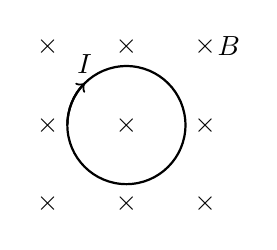
\begin{tikzpicture}
        \foreach \x in {-1,0,1}{
          \foreach \y in {-1,0,1}{
            \node at (\x,\y) {$\times$};
          }
        }
        \draw[thick](0,0) circle(.75);
        \draw[thick,->](-.75,0) arc(180:135:.75) node[above]{$I$};
        \node at (1.3,1) {$B$};
      \end{tikzpicture}
    \end{center}
    \begin{enumerate}[noitemsep,topsep=0pt,leftmargin=18pt,label=(\Alph*)]
    \item The wire loop will rotate clockwise.
    \item The wire loop will rotate counterclockwise.
    \item The wire loop will flip on a horizontal axis through its center.
    \item The wire loop will expand in size.
    \item The wire loop will contract in size.
    \end{enumerate}
    \vspace{.7in}
  \end{enumerate}

  \textbf{Questions \ref{q:circ1}--\ref{q:circ2}}
  A negatively charged particle of mass $m$ and charge $q$ in a uniform magnetic
  field $B$ travels in a circular path of radius $r$.
  \begin{center}
    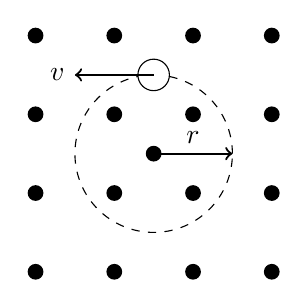
\begin{tikzpicture}
      \foreach \x in {0,...,3}{
        \foreach \y in {0,...,3}{
          \fill[black](\x,\y)circle(.1);
        }
      }
      \fill[black](1.5,1.5)circle(.1);
      \draw[thick,->](1.5,1.5)--(2.5,1.5) node[midway,above]{$r$};
      \draw[dashed](1.5,1.5) circle(1);
      \draw[fill=white](1.5,2.5) circle(.2);
      \draw[thick,->](1.5,2.5)--(.5,2.5) node[left]{$v$};
    \end{tikzpicture}
  \end{center}
  \begin{enumerate}[leftmargin=18pt,resume]
  \item In terms of the other given quantities, the charge-to-mass ratio $q/m$
    of the particle is
    \begin{enumerate}[nosep,leftmargin=18pt,label=(\Alph*)]
    \item $\displaystyle\frac{Bv}{r}$
    \item $\displaystyle\frac{r}{Bv}$
    \item $\displaystyle\frac{rv}{B}$
    \item $rvB$
    \item $\displaystyle\frac{v}{rB}$
    \end{enumerate}
    \label{q:circ1}
    
  \item The work done by the magnetic field after two full revolutions of the
    charge is
    \begin{enumerate}[nosep,leftmargin=18pt,label=(\Alph*)]
    \item zero
    \item $-qvB/rm$
    \item $qvm/Br$
    \item $-mBr/qv$
    \item $-mqvBr$
    \end{enumerate}
    \label{q:circ2}
    \columnbreak
    
  \item A dynamic microphone contains a magnet and a coil of wire connected to
    a movable diaphragm, as shown in the figure. Sound waves directed at the
    diaphragm generate a current in the wires leading from the coil. Which of
    the following helps to explain why this occurs?
    \begin{center}
      \pic{.4}{mic}
    \end{center}
    \begin{enumerate}[nosep,leftmargin=18pt,label=(\Alph*)]
    \item The area of the coil changes.
    \item The magnitude of the magnetic field produced by the magnet changes.
    \item The angle between the plane of the coil and the magnetic field
      produced by the magnet change.
    \item The strength of the magnetic field in the plane of the coil changes.
    \end{enumerate}
    \vspace{.7in}
      \item A current is passed through an analog ammeter and the needle moves
    to indicate the current flowing through the circuit. Which of the
    following best explains how an analog ammeter works?
    \begin{enumerate}[nosep,leftmargin=18pt,label=(\Alph*)]
    \item Current is passed through the needle placed in a magnetic field,
      and the needle is attracted to the high side of the scale.
    \item The needle is a magnet, and is attracted to a magnet on the high
      side of the scale.
    \item The needle gathers an electrostatic charge from the current, and is
      attracted to an electrostatic charge on the high side of the scale.
    \item Current is passed through a spring coil of wire placed in a
      magnetic field, and the coil rotates, moving the needle
      proportionally to the current in the coil.
    \item Current flows through the needle, making it heavier, and it falls to
      the high side of the scale.
    \end{enumerate}
    \vspace{.7in}
    
  \item An electric motor consists of a current-carrying loop of wire mounted
    to an axle and turned at a slight angle in a magnetic field as shown. The
    wire loop will
    \begin{center}
      \pic{.35}{motor-drawing}
    \end{center}
    \begin{enumerate}[nosep,leftmargin=18pt,label=(\Alph*)]
    \item experience a torque and turn clockwise
    \item experience a torque and turn counterclockwise
    \item accelerate upward out of the magnetic field
    \item accelerate downward out of the magnetic field
    \item not experience a force or torque
    \end{enumerate}
  \end{enumerate}
\end{multicols*}
\newpage

\genfreetitle{2}{MAGNETISM}{5}

\genfreedirections

\vspace{.3in}
\begin{center}
  \begin{tikzpicture}[american voltages,scale=1.4]
    \begin{scope}[thick]
      \draw(1.5,0)--(0,0) to[battery,l=$\mathcal{E}$] (0,2)--(1.5,2);
      \draw(1.5,1.9) rectangle(8,2.1);
      \draw(1.5,-.1) rectangle(8,.1);
      \draw[<->](7.5,.1)--(7.5,1.9) node[midway,left]{$d$};
      \draw(1.1,1) circle(.1) node[above]{$m$} node[below left]{$q$};
      \draw[->](1.2,1)--(2,1) node[right]{$v$};
    \end{scope}
  \end{tikzpicture}
\end{center}
\begin{enumerate}[leftmargin=15pt]

\item A positively charged particle ($q$) of mass $m$ travels horizontally,
  with a velocity of $v$, through the center of two capacitor plates. The
  plates areseparated by a distance of $d$ and connected to a battery of
  potential difference ($\mathcal{E}$), as shown in the figure.
  \begin{enumerate}
  \item Sketch the electric field between the plates.
  \item Derive an algebraic expression for the electric field between the
    plates in terms of given quantities. Show all your work.
  \item Describe the motion of the particle as it passes through the capacitor
    plates. What shape is the path? Which direction is the acceleration?
  \item What direction of magnetic field is needed to make the particle travel
    horizontally straight through the capacitor plates?
  \item Derive an algebraic expression for the magnitude of the magnetic field
    needed to cause this straight, horizontal motion between the plates in
    terms of given quantities. Show all your work.
  \item The crossed electric and magnetic fields are adjusted to cause
    positively charged particles with a velocity of vto travel straight. What
    happens to a particle traveling at $2v$? Will it travel straight, or will it
    curve? If it curves, indicate which way it will curve, and explain why.
    If it continues to travel straight, explain why.
  \item The crossed electric and magnetic fields are tuned to cause positively
    charged particles with a velocity of vto travel straight. What happens
    to a negatively charged particle traveling at v? Will it travel straight, or
    will it curve? If it curves, indicate which way it will curve, and explain
    why. If is continues to travel straight, explain why.
  \end{enumerate}
  \newpage
  
  \begin{center}
    \begin{tikzpicture}
      \foreach\x in {0,...,5}{
        \foreach\y in {0,...,5}\fill(\x,\y) circle(.1);
      }
      \draw[thick](6,.5) --(-2,.5) to[R,l=$R$] (-2,4.3)--(6,4.3);
      \draw[thick,<->](5.7,.5)--(5.7,4.3) node[midway,right]{$y$};
      \fill(1.4,0.3) rectangle(1.6,4.6);
      \draw[very thick,->](.5,2.5)--(3.8,2.5) node[right]{$v$};
      \draw[thick,<->](-2,-.3)--(1.5,-.3) node[midway,below]{$x$};
      \node at(4.5,5.4){$B$};
    \end{tikzpicture}
  \end{center}
\item Two long parallel wires, separated by a distance of $y$, pass through a
  region of magnetic field ($B$). The two wires are connected by a resistor
  ($R$) and a metal bar, separated by a distance of $x$, to produce a circuit
  loop, as shown in the figure. The metal bar slides along the wires to
  the right at a velocity of $v$.
   \begin{enumerate}
   \item Calculate the induced emf ($e$) in the bar in terms of the given
     quantities.
   \item Calculate the current in the circuit in terms of the given quantities.
   \item What is the direction of the current in the resistor--upward or
     downward?
   \end{enumerate}
\end{enumerate}
\end{document}
